%
% Qualitative example of switch bouncing versus CPU clock.
%
\documentclass[border=3mm]{standalone}
\usepackage{tikz}
\usetikzlibrary{circuits.ee.IEC}

\begin{document}

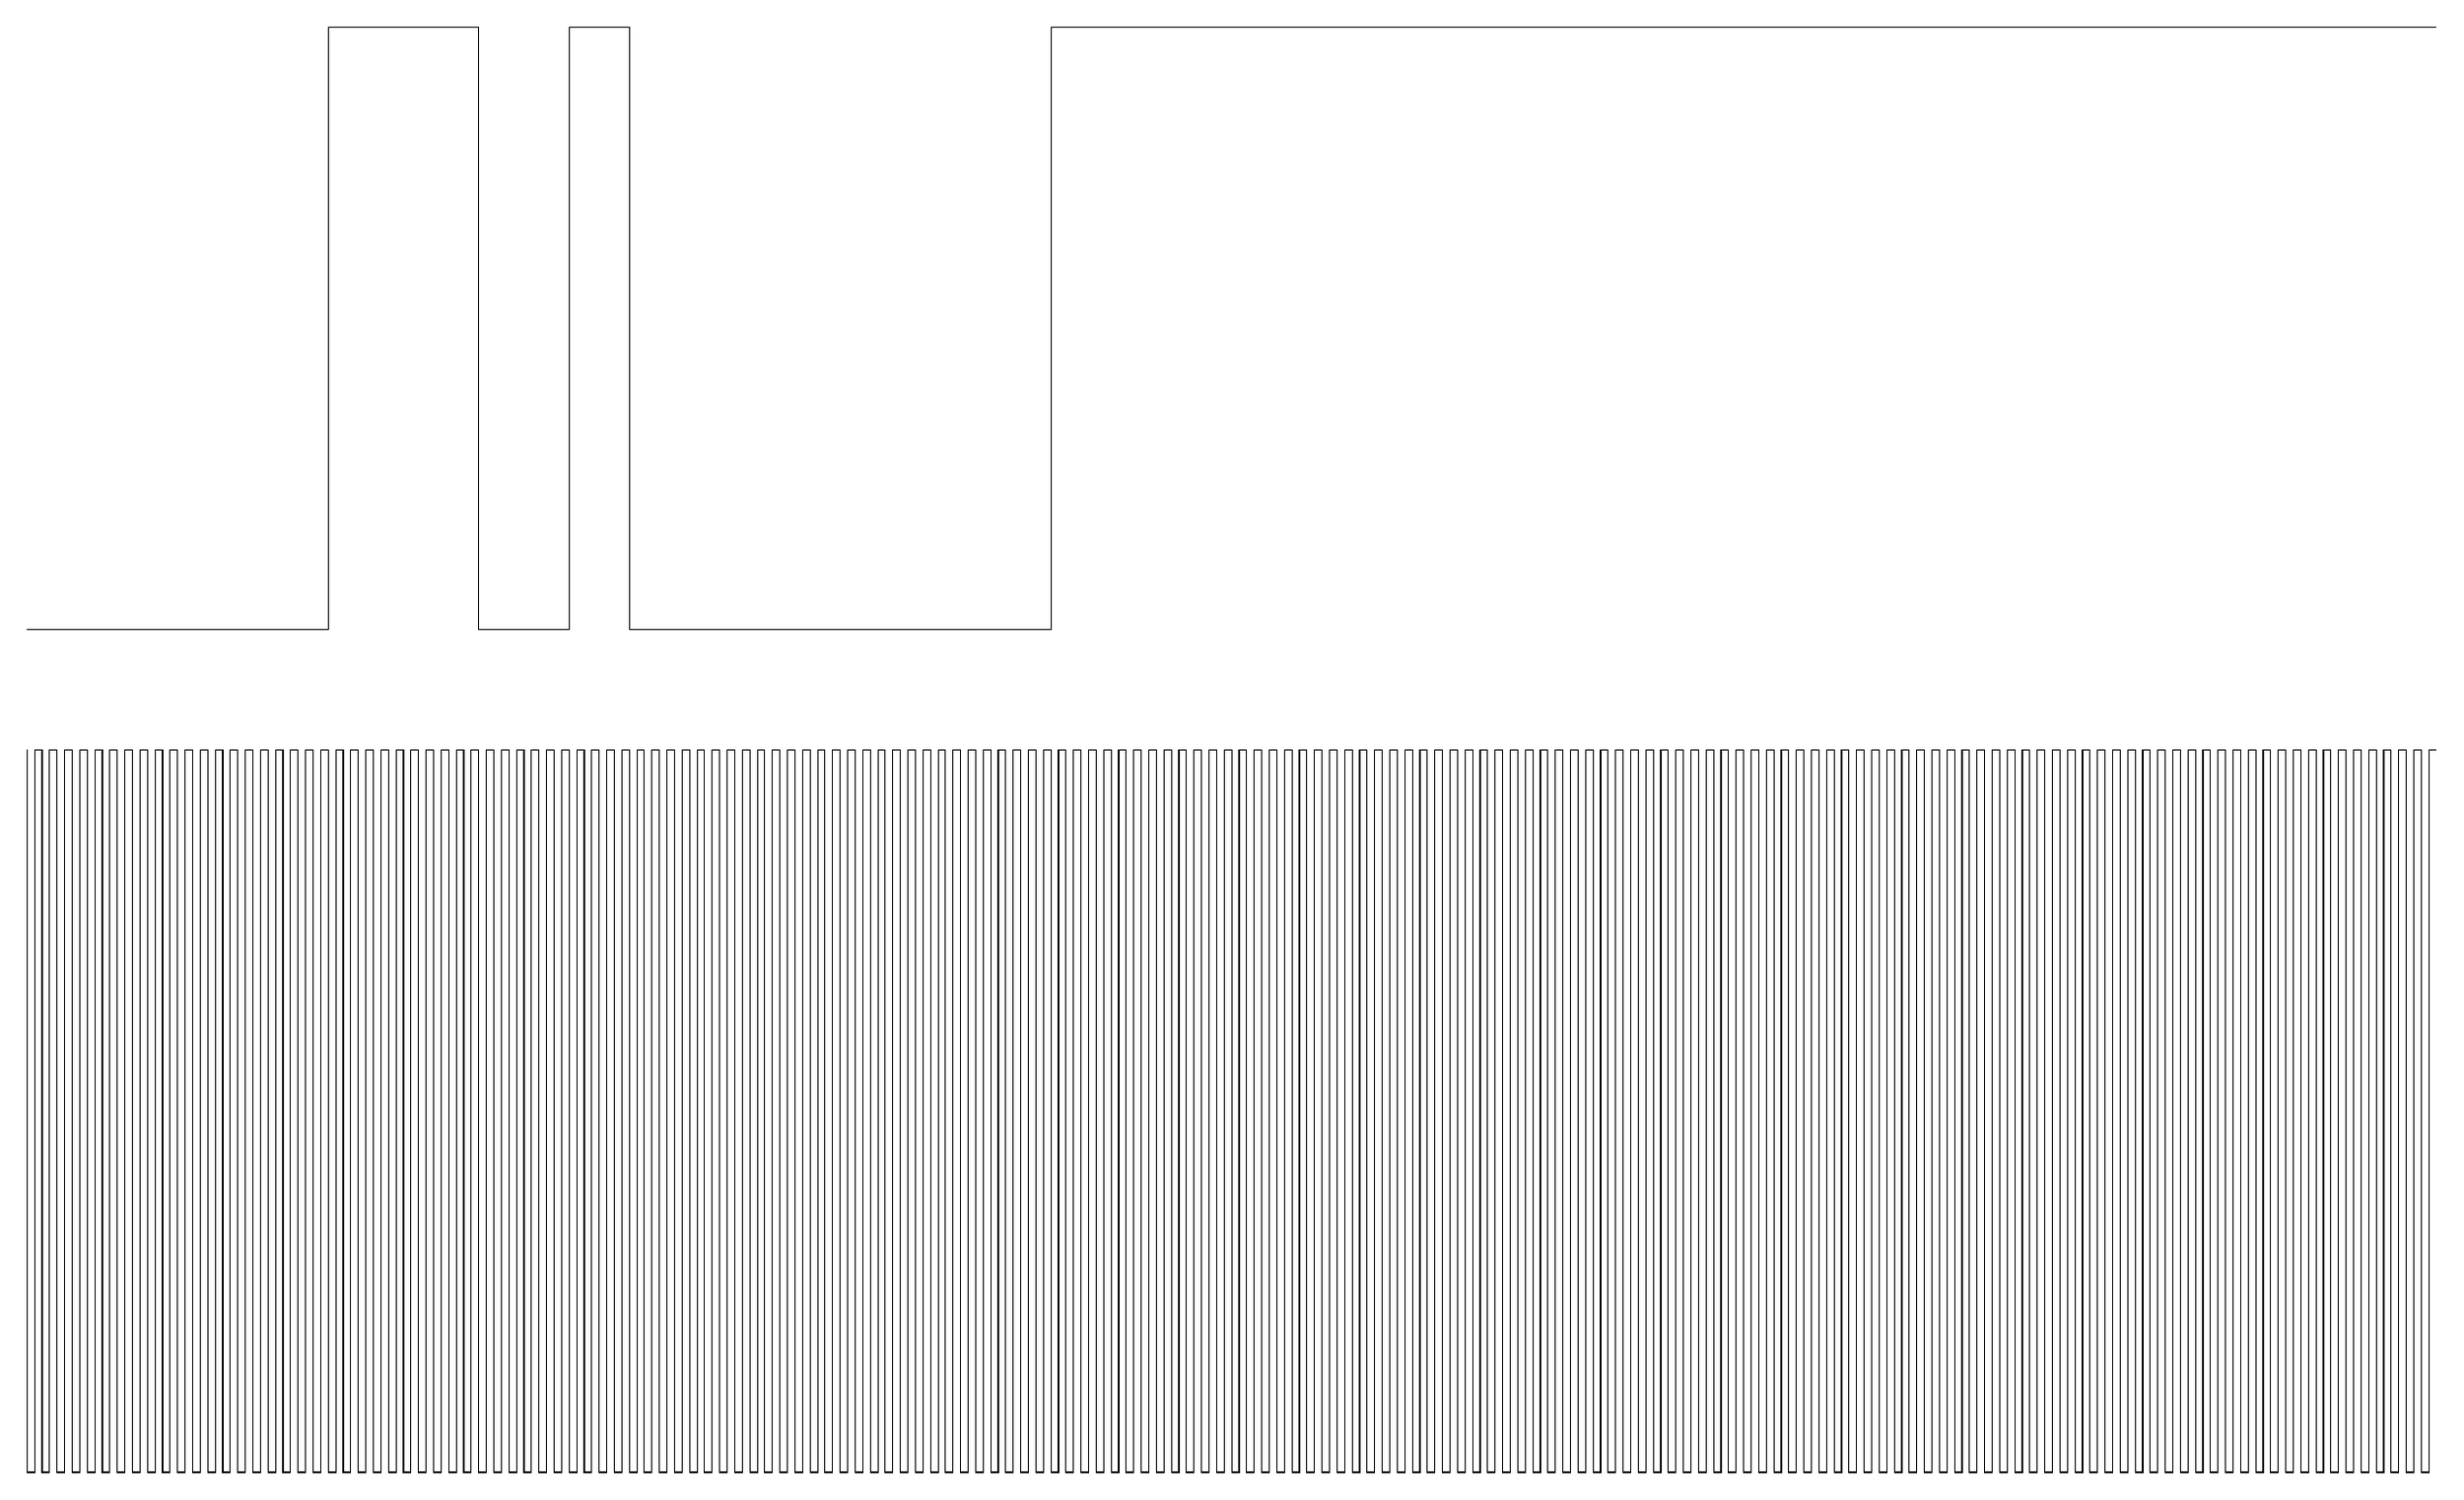
\begin{tikzpicture}
    \draw [-] (0,0)
        to (4.0,0) to (4.0,8)
        to (6,8) to (6,0)
        to (7.2,0) to (7.2,8)
        to (8,8) to (8,0)
        to (13.6,0) to (13.6,8)
        to (32,8);
    \foreach \x [evaluate=\x as \inieval using 2*\x] in {0,0.1,...,16}
        \draw[thin] (\inieval,-1.6) -- ++(0,-9.6) -| (\inieval+0.1,-1.6) -- (\inieval+0.2,-1.6);
\end{tikzpicture}

\end{document}

